\documentclass[12pt]{article}
\usepackage{graphicx}
\graphicspath{ {./figures/} }

\title{Final Report:\\ Neuroevolution of Task Specialisaiton for Multi-Agent Systems}
\author{Mostafa Rizk}

\setlength{\parindent}{0pt}

\begin{document}

\maketitle

\section{Introduction}

\section{Landscape Analysis}

\textbf{What are the fundamental features of the fitness landscape of a task specialisation problem?}\\

\subsection{Creating a Fitness Gradient}

One conclusion of the research so far has been that the landscape of task specialisation problems appears to be very flat and thus difficult to find any solution at all, let alone a specialised one.
If a flat fitness landscape is inherent to task specialisation problems, then this is significant because it implies that algorithms that are highly exploratory should be used, as they are with similar problems \cite{oller:AAMAS:2020}.
However, it is also possible that the fitness function might be making evolution unnecessarily difficult because it only rewards task completion, treating partial success the same as failure.
If partial successes are rewarded, the landscape could have a smoother gradient, making it easier for evolution to traverse.
This leads to the following hypothesis:\\

\textbf{Hypothesis 1.1:} Rewarding agents for partial retrieval of the resource will create a smoother fitness gradient.\\

This hypothesis is answered by conducting the following experiment:\\

\textbf{Experiment 1.1- RWG Analysis with Modified Fitness:}  Modify the fitness function such that agents are rewarded for partially retrieving a resource.
Specifically, divide the reward for retrieving a resource by the length of the arena and give agents part of the reward if they move the resource a single tile closer to the goal.
Then conduct RWG analysis as described in \cite{oller:AAMAS:2020} and compare the plots to those produced for the original fitness function.\\

If the mean curve of the distribution has a smoother gradient, then the hypothesis is supported.\\

The plots for the original landscape analysis and the analysis with the new fitness function are shown in Figure \ref{fig:sparse} and Figure \ref{fig:incremental} respectively.\\

\begin{figure}[h]
\centering
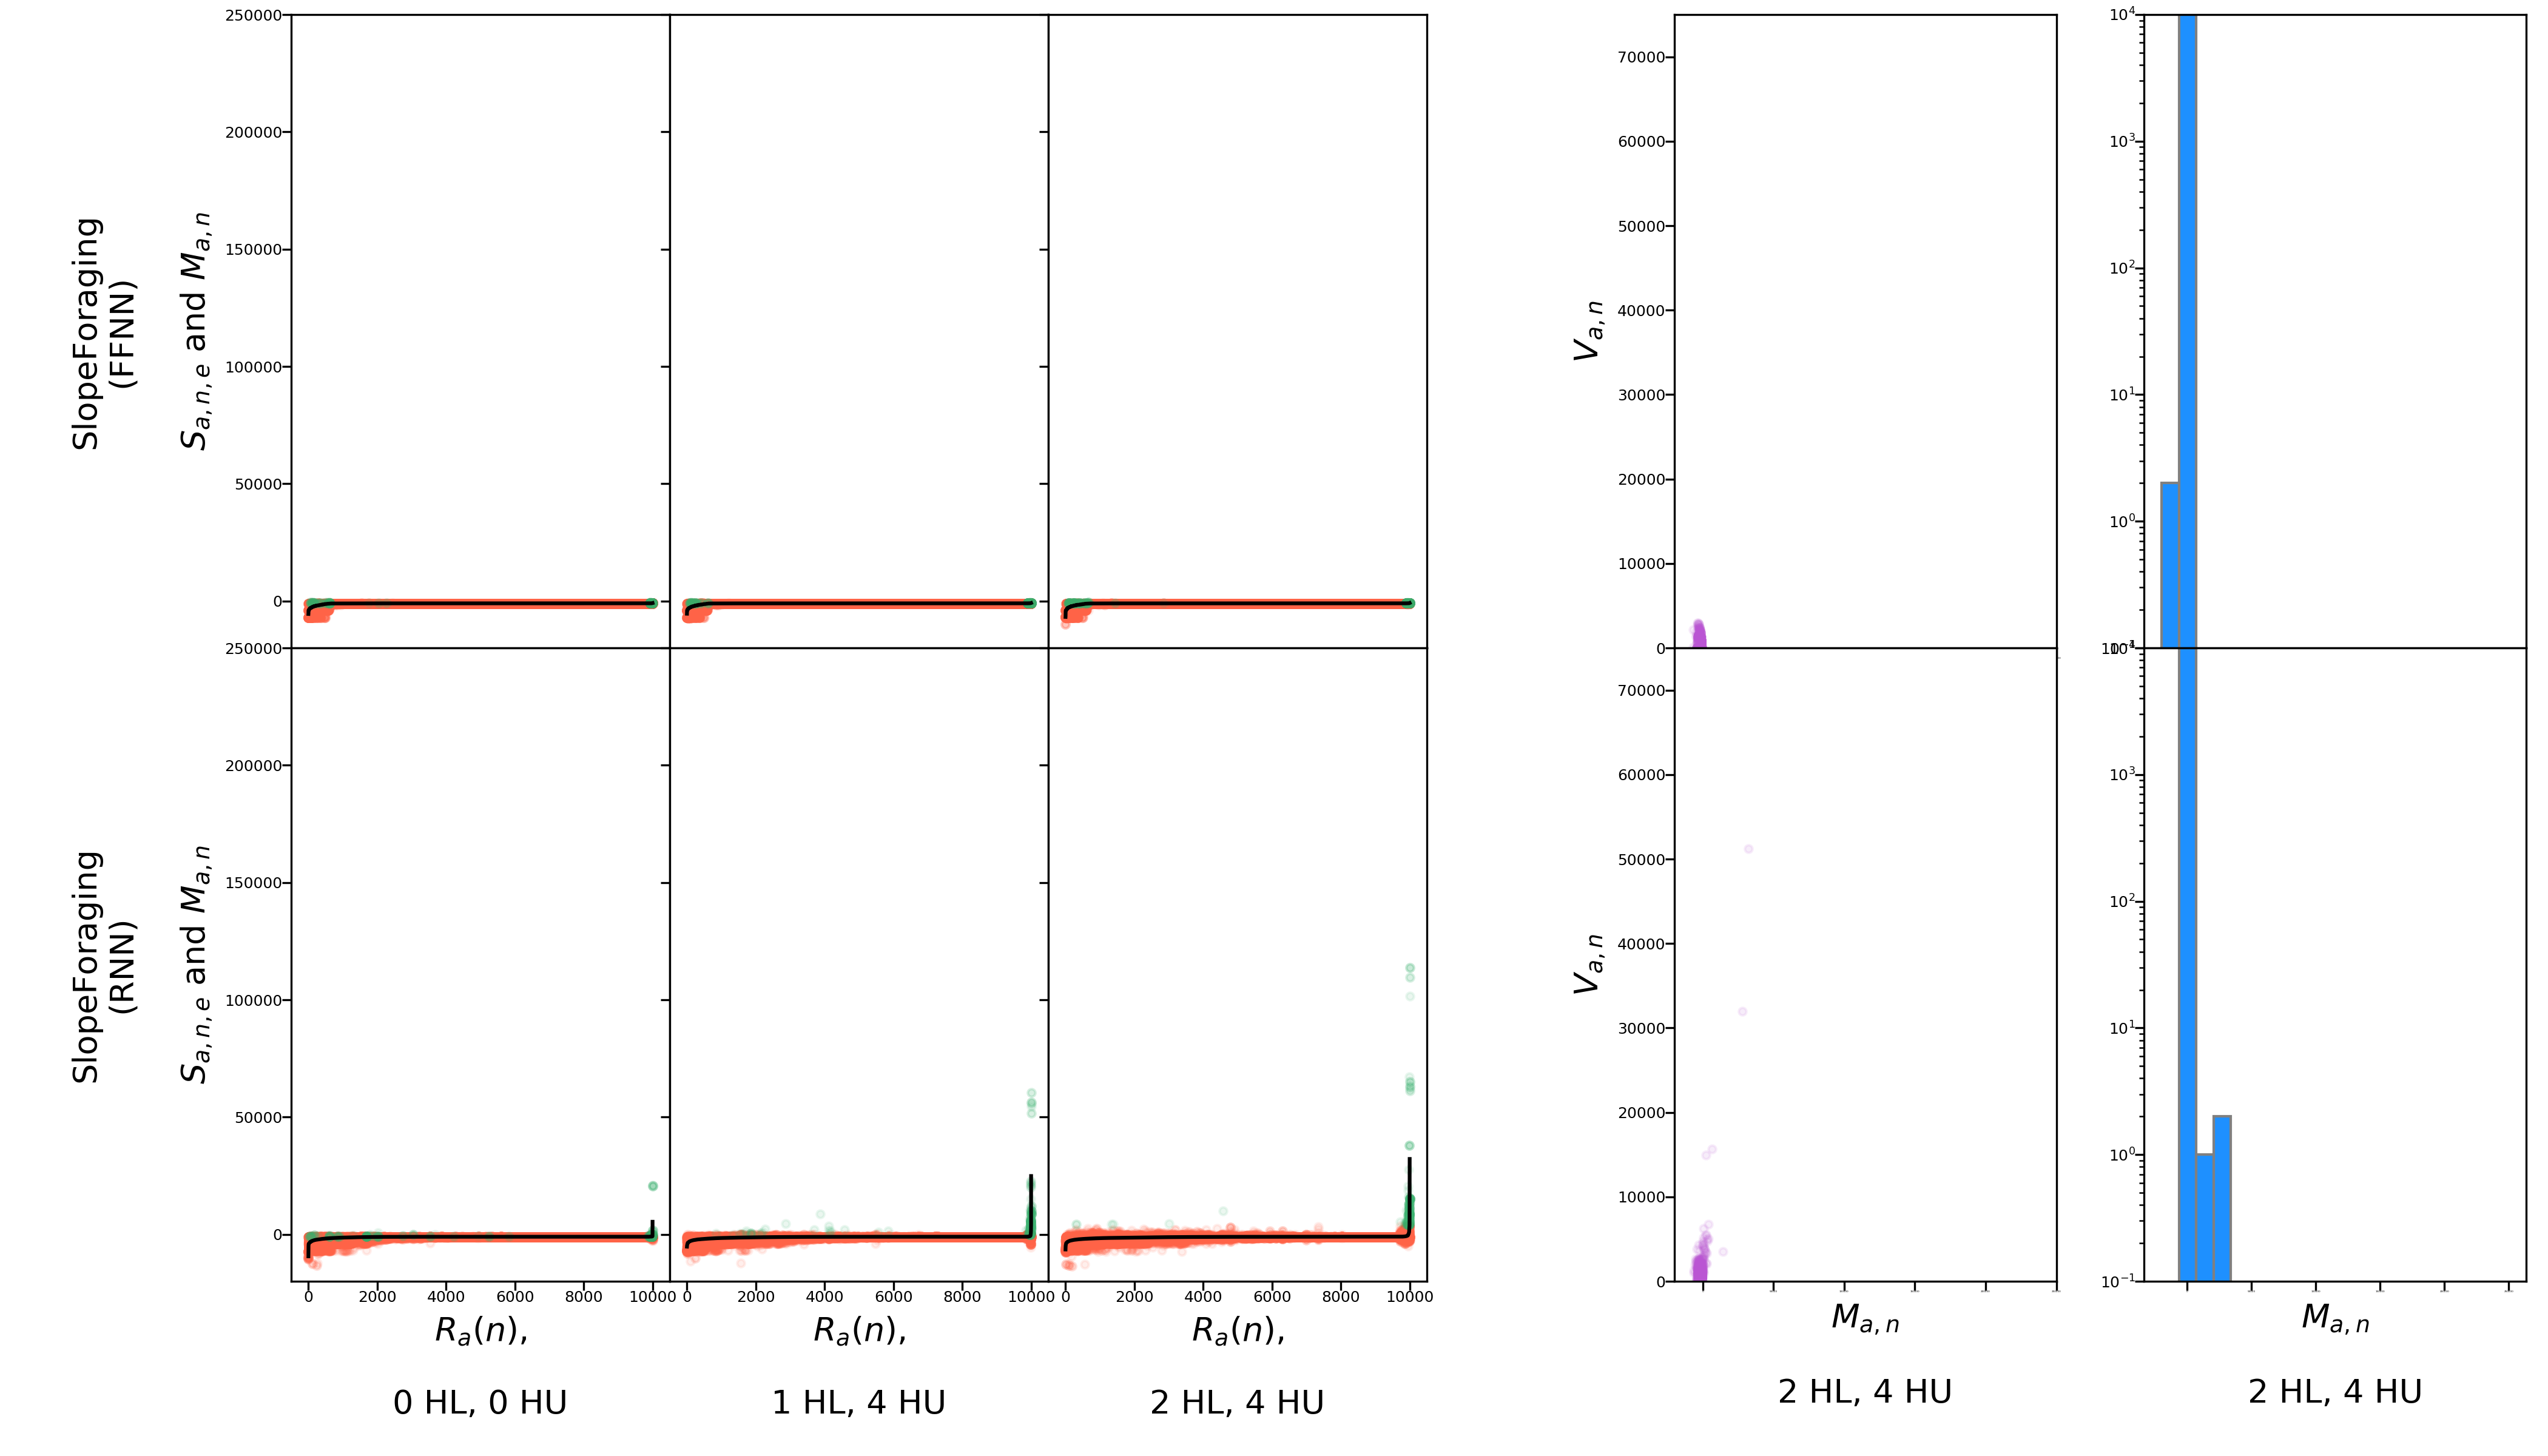
\includegraphics[width=1.0\textwidth]{sparse_rewards.png}
\caption{RWG Analysis with the original fitness function}
\label{fig:sparse}
\end{figure}

\begin{figure}[h]
\centering
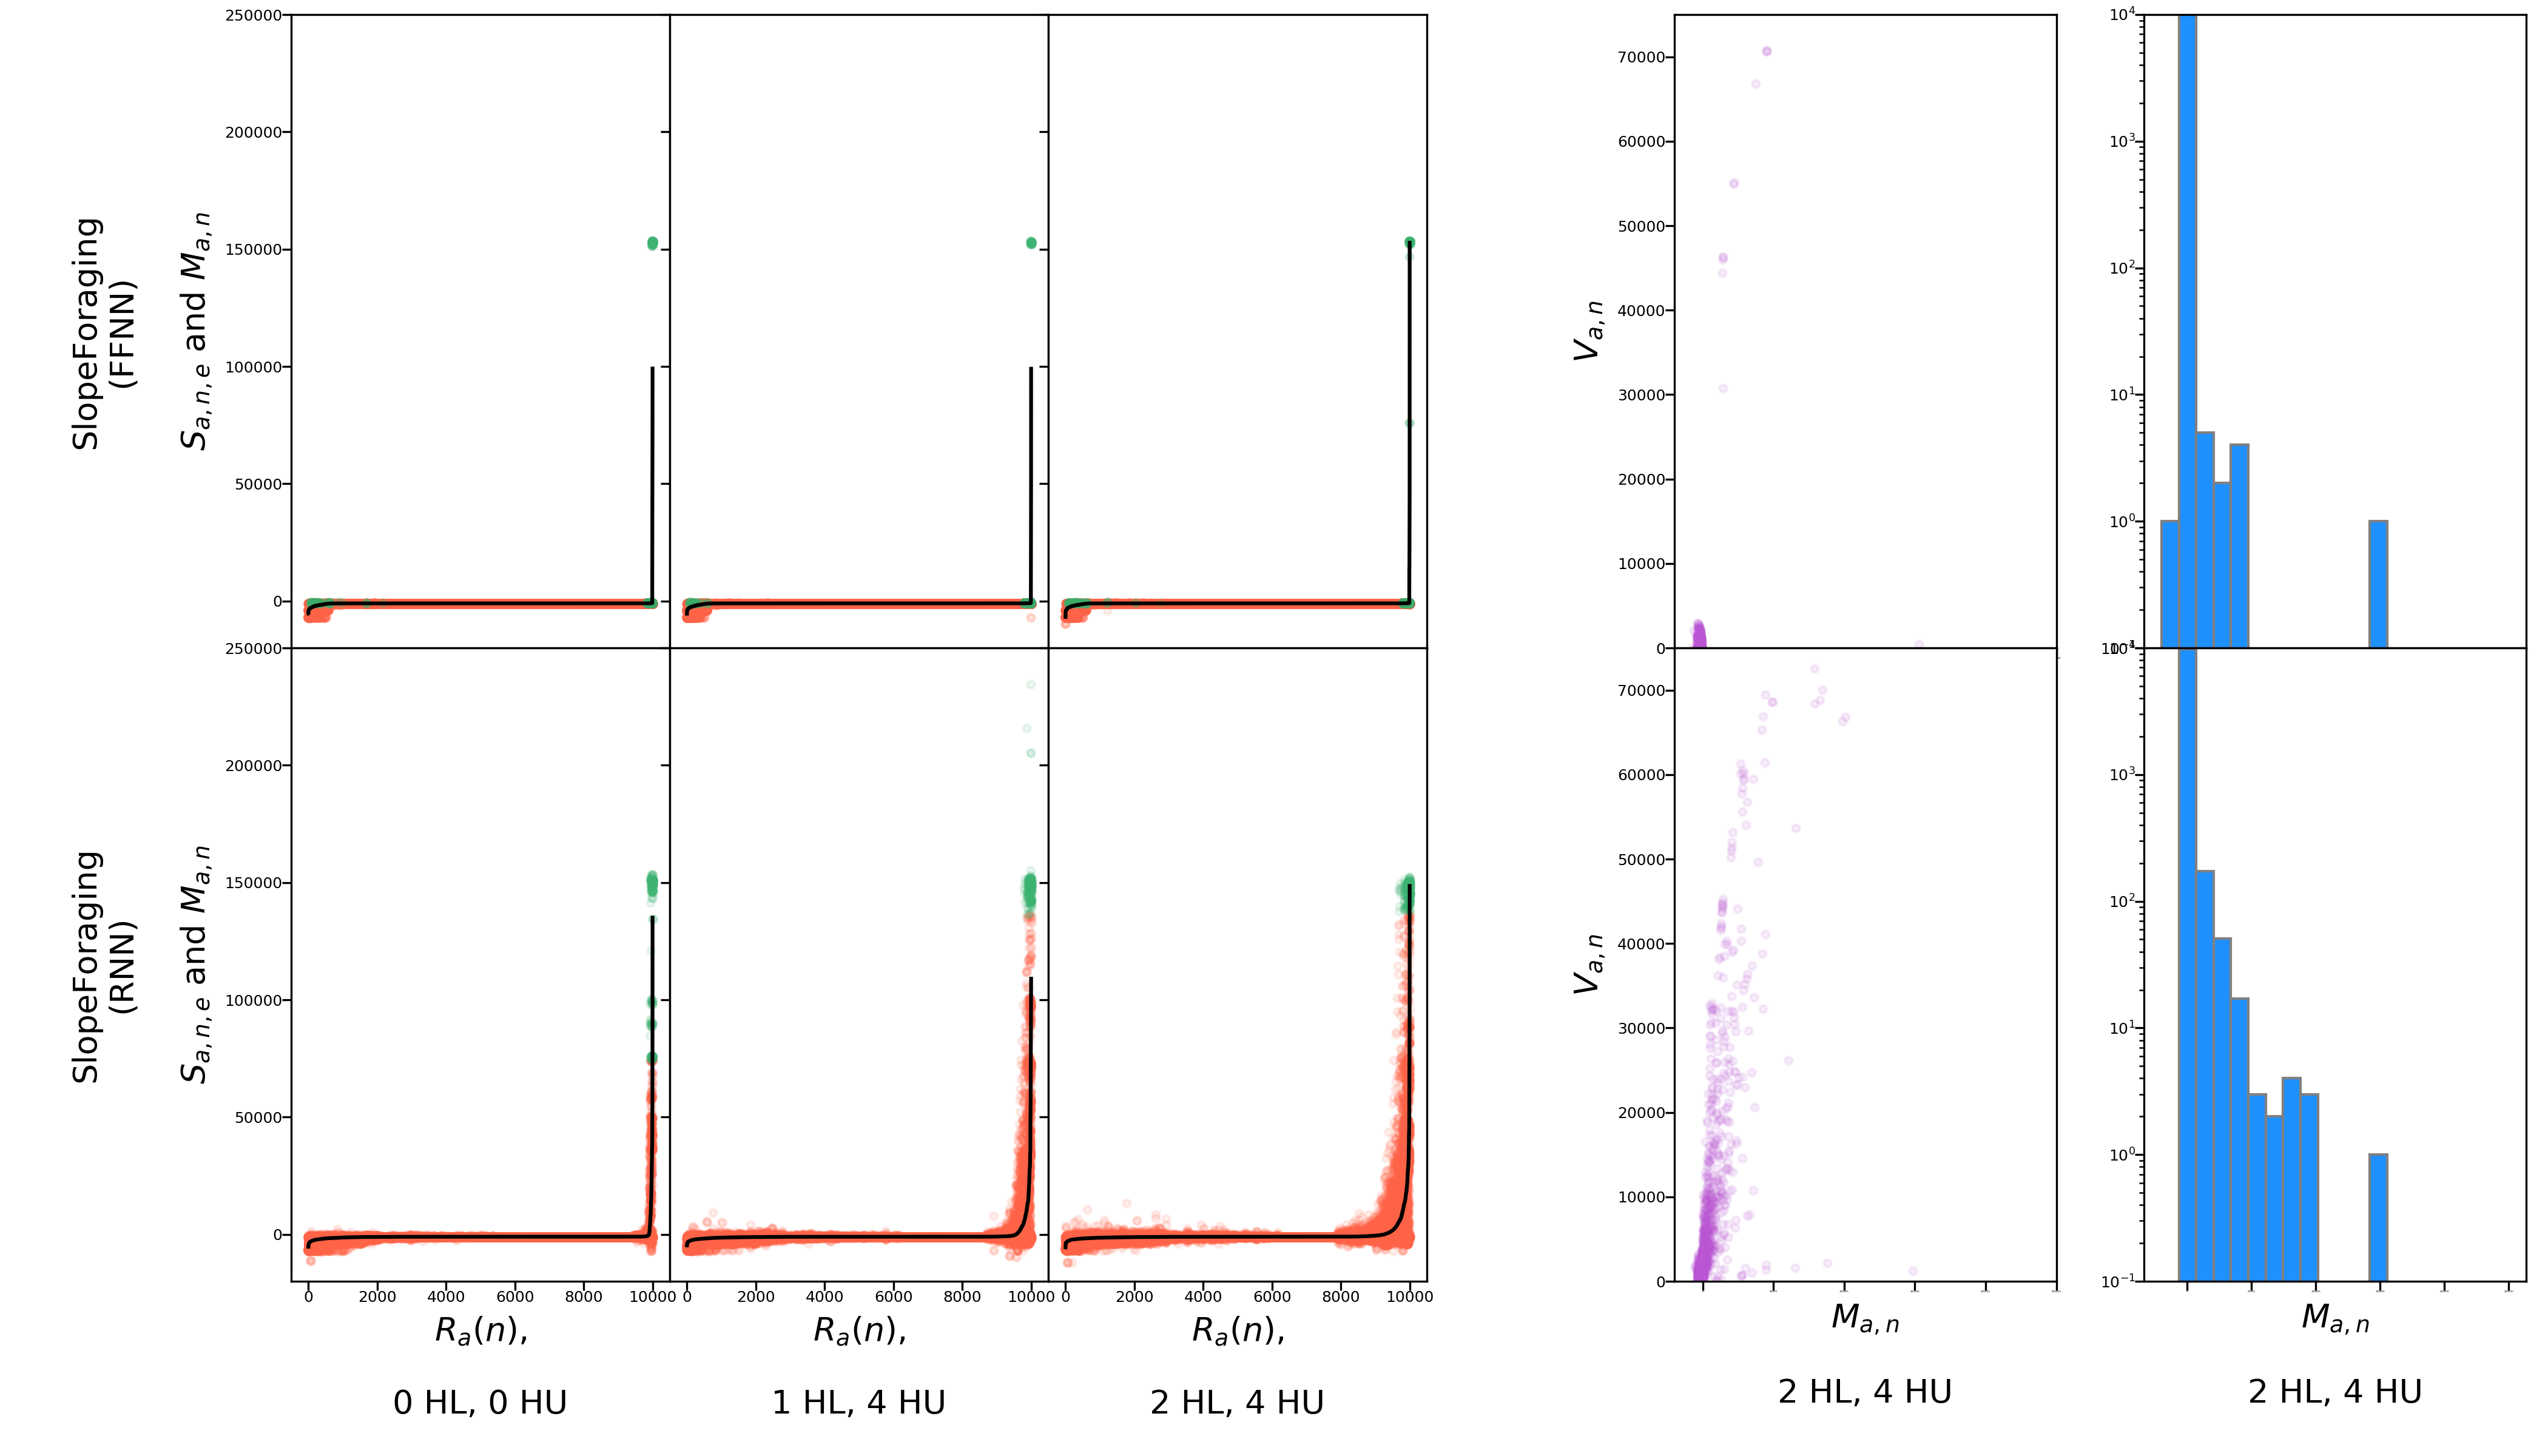
\includegraphics[width=1.0\textwidth]{incremental_rewards.png}
\caption{RWG Analysis with incremental rewards}
\label{fig:incremental}
\end{figure}

Looking at the 6 mean plots in Figure \ref{fig:incremental} compared to Figure \ref{fig:sparse}, we see that with incremental rewards, the solutions do in fact form more of a gradient towards the right end of the plot, in particular for RNNs (bottom row). 
This means that a lot of the solutions in the landscape are partially successful at retrieving resources. 
However, the landscape is still largely flat. 
This is presumably because most solutions in the landscape don't even get to the point of picking up a resource from the source.\\ 

Thus the answer to Hypothesis 1.1 is:\\

\textbf{Answer 1.1:} Rewarding agents for partial retrieval of the resource creates a smoother fitness gradient, but the landscape is still largely flat.\\

In order to further smooth the fitness landscape there would need to be rewards for partial progress up the slope, but the problem with this is that it is likely to disincentivise the collector behaviour in evolution.
Why would an agent stay at the nest and collect resource when they are rewarded for going up the slope? 
Additionally, while this problem is simple enough to smooth the fitness gradient in this way, such smoothing may not be possible for other more complex problems.
The purpose of this research is to understand how to use AI to find good solutions with minimal (if any) human intervention.\\

Moreover, the flatness of the landscape is, to some extent, inherent to this task.
This is a problem common in evolutionary computation known as the bootstrapping problem \cite{Silva:EC:2016, Wei:ALR:2019}.
Bootstrapping is "when the task is too demanding for the fitness function to apply any meaningful selection pressure on a randomly generated population of initial candidate solutions" \cite{Silva:EC:2016}.
The bootstrapping problem often occurs when the goal behaviour is complex relative to the very simple available actions \cite{Wei:ALR:2019}.
For this problem, the available actions are primitives like 'move forward one tile' and 'move backward one tile'.
When putting together sequences of these actions, most sequences will obviously not be very successful.\\

There are many proposed solutions to solving the bootstrapping problem and they fall under the broad categories of inserting human knowledge into the learning process or increasing the diversity of solutions \cite{Silva:EC:2016}.
Smoothing the landscape falls under the former category, but this family of techniques has some shortcomings, in particular it reduces the potential for automation and risks the experimenter introducing negative biases.
Using rwg to find a seed falls under the second category; it has the shortcoming of additional computation, which may not scale well for problems with larger solution spaces, but for those problems there is a wealth of alternative techniques for increasing diversity, such as novelty search.
In keeping with the spirit of AI, I have chosen to continue using the more challenging fitness function.

\subsection{Visualising Specialisation}

I already performed the initial analysis of the landscape (Figure \ref{fig:sparse}), however, the visualisation did not contain any information about how specialised each team was i.e. was a given solution a pair of generalists or a pair of specialists? 
Are the better solutions in the landscape usually specialists? 
To visualise this information I need a way of measuring the degree of specialisation of a solution, so the second task in this group is to evaluate some candidate metrics and the third is to incorporate the chosen metric into the landscape analysis.
The hypothesis and experiment are:\\

\textbf{Hypothesis 1.2:} Specialist solutions outperform generalist ones.\\

\textbf{Experiment 1.2- Specialisation Plots of RWG Analysis:}  Use the chosen specialisation metric to assess all the solutions found by RWG analysis and incorporate them into the plots.\\

The most specialised solutions are expected to be at the rightmost of the mean plot and above the generalist ones.
If this is the case, then it supports the hypothesis.
If there are generalist solutions that outperform specialist ones, it disproves the hypothesis.

\subsubsection{Choosing a Metric}

\subsubsection{Results}

\subsection{Dimensionality Reduction}

The neural networks used to solve the Slope Foraging problem have hundreds of weights, meaning that the fitness landscape has just as many dimensions and is consequently very difficult to visualise.
Reducing the dimensionality of the problem to two or three dimensions makes visualisation possible and gives many valuable insights into the features of the landscape, especially if combined with a specialisation metric.
How far apart are specialist and generalist solutions in the landscape?
How many optima are there?
What trajectory does evolution take through the landscape?
There are many techniques to choose from \cite{veerapen:GPEM:2018} and further consideration is necessary before choosing one, but Sammon mapping \cite{sammon:IEEETR:1969} is currently the preferred method due to its ability to preserve the relative distances between solutions and its use in other agent-based and neuroevolution studies \cite{kim:GECCO:2003, risi:AB:2010}.

The hypothesis is:\\

\textbf{Hypothesis 1.3:} There are two optima in the landscape, one composed of specialist solutions and one composed of mostly generalist solutions. \\

\textbf{Experiment 1.3- Dimensionality Reduction:} Assemble a dataset of solutions, combining some random ones from rwg and some evolved ones.
Apply the chosen dimensionality reduction technique to the dataset.
Use the chosen specialisation metric to plot the degree of specialisation (in addition to the fitness).\\

If there are indeed two optima, then the hypothesis is supported, otherwise it is not supported.
If, additionally, the specialist solutions are fitter than the generalist ones, Hypothesis 1.2 is further supported.\\

\begin{figure}[h]
\centering
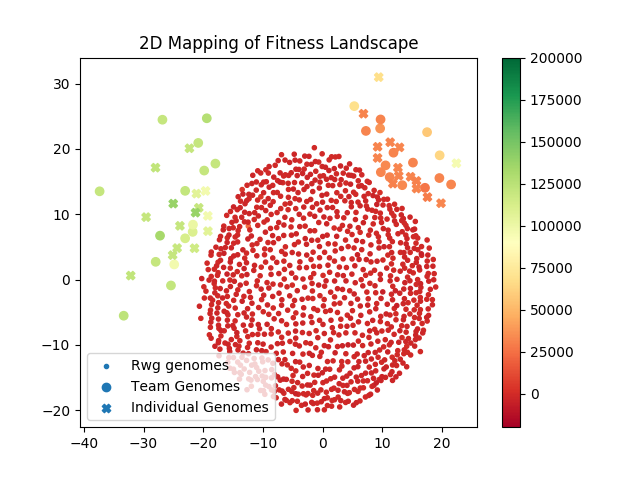
\includegraphics[width=1.0\textwidth]{sammon.png}
\caption{Sammon Mapping of Landscape}
\label{fig:sammon}
\end{figure}

The algorithm I use to perform dimensionality reduction creates an initial 2D mapping of the genomes and calculates the error of that mapping using Sammon's error function. 
It then uses iterative gradient descent to minimise the error. 
The plot in Figure \ref{fig:sammon} includes the best 500 and worst 500 genomes from the rwg analysis in Figure \ref{fig:sparse} along with the best evolved team genomes and the best evolved individual genomes. 
For the individual genomes, I concatenated two identical copies and doubled their score so that I can put them in the same landscape.\\

Preliminary results show that there indeed appear to be two optima, which supports Hypothesis 1.3.
One of the optima has a higher score while the other has a lower score.
Anecdotally, the scores observed for the green optima are usually only seen for teams of specialists, however a specialisation metric is still needed to verify this empirically.\\

\subsection{Analysis of Different Slope Angles}

\textbf{Hypothesis 1.4.1:} When the slope is flat, there will only be one optima of generalists and no specialist solutions.\\

\textbf{Hypothesis 1.4.2:} An intermediate slope will have two optima (one specialist and one generalist).\\

\textbf{Hypothesis 1.4.3:} The specialist solutions will outscore the generalists, but the disparity will be smaller than the steeper slope setting. \\

\textbf{Experiment 1.4- RWG with Different Slope Angles:} Repeat RWG, as it was done for previous experiments, but with no slope and intermediate slope.
Then perform 30 evolutionary runs, each with a different seed genome and random seed.
Use the generated data to create RWG analysis plots and perform dimensionality reduction.\\

\subsection{Decentralised Solutions} 

\textbf{Hypothesis 1.5:} Solutions found by the decentralised algorithm will be primarily generalist whereas solutions found by the centralised algorithm will be primarily specialist.\\

\textbf{Experiment 1.5- Decentralised Dimensionality Reduction:} Perform 30 evolutionary runs of the decentralised setup.
Calculate the degree of specialisation of all evolved solutions.
Concatenate the genomes of all individuals on a team and apply dimensionality reduction to the data.
Combine the decentralised data with the centralised data and plot on the same plot.\\

\section{Centralised vs Decentralised Solutions}

\textbf{When do centralised and decentralised solutions outperform one another in task specialisation problems?}\\

\subsection{Scalability}

\textbf{Hypothesis 2.1.1:} If evolution is run with larger team sizes, the fitness of centralised solutions will decrease.\\

\textbf{Hypothesis 2.1.2:} If evolution is run with larger team sizes, the fitness of decentralised solutions will decrease less rapidly than centralised solutions\\

\textbf{Hypothesis 2.1.3} If evolution is run with larger team sizes, the centralised approach will find fewer specialists.\\

\textbf{Hypothesis 2.1.4} If evolution is run with larger team sizes, the decentralised approach will find the same number of specialists.\\

\textbf{Experiment 2.1- Evolution with Larger Teams:} Do 30 evolutionary runs (centralised and decentralised) for teams of 4, 6, 8 and 10 agents.
Calculate the specialisation of all evolved solutions.
Plot the average fitness per agent and team specialisation for teams in each setup. \\

\subsection{Robustness}

\textbf{Hypothesis 2.2.1:} When evolved teams have team-members replaced, the average fitness per agent decreases for centralised teams.\\

\textbf{Hypothesis 2.2.2:} When evolved teams have team-members replaced, the average fitness per agent decreases for decentralised teams, but by a smaller margin than centralised teams.\\

\textbf{Hypothesis 2.2.3:} When evolved teams have team-members replaced, the team specialisation decreases for centralised teams.\\

\textbf{Hypothesis 2.2.4:} When evolved teams have team-members replaced, the team specialisation remains the same for decentralised teams.\\

\textbf{Experiment 2.2- Changing Team-mates:} Take all 60 evolved 2-agent teams (30 centralised + 30 decentralised).
For each evolved team, replace one agent 4 times: once with a dropper, once with a collector, once with a generalist and once with a stationary agent.
Calculate the average fitness and team specialisation then repeat for the other agent on the team.
That is a total of $2 \times 30 \times 4 \times 2= 480 \mbox{ fitness evaluations}$. 
Create a violin plot for the centralised setup and one for decentralised setup.
Draw one violin for the original team and one for each replacement (a total of five).
The data for each violin includes when each of the two agents was replaced.
The y-axis shows the fitness and the plots also have a colour scale to show the degree of specialisation.\\

\section{Theoretical Modelling}

\textbf{What is the price of anarchy in task specialisation problems?}\\

\textbf{Hypothesis 3.1.1:} The slope foraging problem is a stag hunt with two Nash equilibria, where the payoff-dominant equilibrium is specialist solutions and the risk-dominant is generalist solutions.\\

\textbf{Hypothesis 3.1.2:} Socially optimal teams are more likely to converge to the payoff-dominant Nash equilibrum while the self-interested teams are more likely to converge to the risk-dominant Nash equilibrium.\\

\textbf{Experiment 3.1- Game-theoretic Modelling:} Formulate a game that models the experimental setup. 
Find the nash equilibria and study the learning dynamics.\\

\bibliographystyle{ieeetr}
\bibliography{references}

\appendix

\section{Summary of Results}

\begin{description}
\item[1] \textbf{What are the fundamental features of the fitness landscape of a task specialisation problem?}\\

\textbf{Answer 1.1:} Rewarding agents for partial retrieval of the resource creates a smoother fitness gradient, but the landscape is still largely flat.\\

\item[2] \textbf{When do centralised and decentralised solutions outperform one another in task specialisation problems?}\\



\item[3] \textbf{What is the price of anarchy in task specialisation problems?}\\



\end{description}

\end{document}